\chapter{Integration}

We are now ready to begin talking about the integration side of complex calculus. Since complex functions can be thought of as functions of two variables, we have a couple of options for integrating: surface integrals, such as $\int_{U} f(z)dxdy$ where we integrate over the open set $U$; and line integrals $\int_{\gamma} f(z)dz$ where we integrate over a curve $\gamma$ in $\C$.

It turns out that surface integrals hold little interest. Line integrals are where the magic happens. Here are some facts we're going to be able to show using complex line integrals:

\begin{itemize}
\item Every holomorphic function is infinitely differentiable.
\item Every holomorphic function is analytic, meaning it has a power series expansion around any point in the domain.
\item Liouville's theorem states that any bounded entire function is constant.
\item Let $a\in (0,1)$. Then 
$$\int_0^\infty \frac{x^{a - 1}}{1 + x}dx = \frac{\pi}{\sin(\pi a)}$$
\end{itemize}

Liouville's theorem is a neat theoretical tool, which will give us some very powerful theorems. It's going to allow us to prove the Fundamental Theorem of Algebra (every non-constant complex polynomial has roots). 

Why might the last fact be interesting? Well, it's not the fact by itself that's interesting. After all, it's a seemingly random integral. (Indeed, it only holds interest to me because it appeared on my comprehensive exam for complex analysis!) What's interesting is that we can use complex line integrals to find real improper integrals.

\section{Curves in $\C$}

Before we can begin discussing line integrals, we should give ourselves a quick refresher on curves. After all, we need to integrate over {\it something}.

\begin{defbo}{Curves}{curve}\index{Curve}A {\bf curve} in $\C$ is a function $\gamma:[a,b] \rightarrow \C$, for some real $a < b$, such that $\RE(\gamma)$ and $\IM(\gamma)$ are continuous.

\vspace{5pt}

Further, such a curve is called {\bf smooth} if $\RE(\gamma)$ and $\IM(\gamma)$ are differentiable. It is called {\bf piecewise smooth} if they are differentiable except at finitely many places. In this case, $\gamma' = [\RE(\gamma)]' + i[\IM(\gamma)]'$.

\vspace{5pt}

Paths are a special case of curves, where $a = 0$ and $b = 1$.

\vspace{5pt}

The point $\gamma(a)$ is called the {\bf start} of the curve, and $\gamma(b)$ is the {\bf end} of the curve. $\gamma$ is called {\bf closed} if it starts and ends at the same point.
\end{defbo}

We are going to be using a lot of different paths throughout this course. We present a few common ones:

\begin{ex}{}{} Let $z_0,z_1\in \C$. The line segment from $z_0$ to $z_1$ can be described by the curve $\gamma:[0,1]\rightarrow \C$ with:
$$\gamma(t) = tz_1 + (1-t)z_0 = z_0 + t(z_1 - z_0)$$

So, for example, the line segment from $1 - i$ to $5 + 7i$ is given by the curve $\gamma(t) = 1 - i + t(4 + 8i) = (1+4t) + (-1 + 8t)i$.
\end{ex}

\begin{ex}{}{} Let $z_0 \in \C$ and $r\ge 0$. Fix an angle $\theta$. Then travelling along the circle of radius $r$ centered at $z_0$, starting at $\theta$ and travelling once counterclockwise, is done by the curve:
$$\gamma(t) = z_0 + re^{i(\theta + t)}$$

\noin where $t\in [0,2\pi]$.

If we travel clockwise instead, then the formula is $\gamma(t) = z_0 + re^{i(\theta - t)}$.

We will usually start at $\theta= 0$.

Also, notice that these are both closed curves.
\end{ex}

There are a few interesting ways to manipulate and combine curves. These will pop up, so let's give a brief description:

\begin{defbo}{$-\gamma$}{} Let $\gamma:[a,b]\rightarrow \C$ be a curve in $\C$. Then we can define the curve $-\gamma$ which traverses $\gamma$ backwards at the same speed. We define $-\gamma:[a,b] \rightarrow \C$ by:
$$(-\gamma)(t) = \gamma(a + b - t)$$
\end{defbo}

Why $a + b - t$? When looking at $\gamma$, the variable $t$ travels along the interval $[a,b]$ from $a$ to $b$ linearly. Going backwards, we want a linear function $s:[a,b]\rightarrow [a,b]$ so that $s(a) = b$ and $s(b) = a$. I.e., go from $b$ to $a$ linearly. The function $s(t) = a + b - t$ does this. It's linear, $s(a) = a + b - a = b$ and $s(b) = a + b - b = a$.

We can also combine curves, by following one and then the other.

\begin{defbo}{$\gamma_1 + \gamma_2$}{} Suppose $\gamma_1:[a,b] \rightarrow \C$ and $\gamma_2:[c,d] \rightarrow \C$ are two curves such that $\gamma_1(b) = \gamma_2(c)$. I.e., the second curve starts where the first one ends.

Then $\gamma_1 + \gamma_2$ is the curve that first follows $\gamma_1$ and then follows $\gamma_2$. We define $\gamma_1 + \gamma_2:[a, b + (d-c)]\rightarrow \C$ by:
$$(\gamma_1 + \gamma_2)(t) = \begin{cases} \gamma_1(t), & t\in [a,b]\\
\gamma_2(c -b + t), & t\in [b,b + (d-c)]\end{cases}$$
\end{defbo}

The first part simply says to follow $\gamma_1$ until the end. The second part, however, looks confusing. Why $c-b + t$? Well, keep in mind that when we are done travelling $\gamma_1$, we are at $t = b$. To start $\gamma_2$, we need the input of $\gamma_2$ to be $c$. The formula $c-b + t$ gives $(\gamma_1 + \gamma_2)(b) = \gamma_2(c - b + b) = \gamma_2(c)$, like we want.

And then we end at $b + (d-c)$ since it gives $(\gamma_1 + \gamma_2)(b + (d-c)) = \gamma_2(c - b + (b +(d-c)) = \gamma_2(d)$, also as desired.

These are mostly academic formulas. They'll let us prove some things, and that's their only real use. In fact, we are very quickly going to prove a couple of theorems that render these formulas totally useless.

Lastly, we need to quickly talk a bit about closed curves. As it turns out, here's some notion of "direction" when you travel along a closed curve, provided that it doesn't self intersect. 

\begin{defbo}{Simple Closed Curve}{}\index{Curve!simple closed}
A closed curve is called simple if it does not self-intersect. This means that $\gamma(t) = \gamma(s)$ occurs only when $t = s$ or at the start and end.
\end{defbo}

\begin{thmbo}{Jordan Curve Theorem}{} Let $\gamma$ be a simple closed curve in $\C$. Then $\gamma$ divides $\C$ into two regions: the {\bf inside} and {\bf outside} of $\gamma$. We shall denote these $\mathrm{in}(\gamma)$ and $\mathrm{out}(\gamma)$.

The outside of $\gamma$ consists of all points $z\in \C$ such that there exists a path from $z$ to $\infty$ that does not cross $\gamma$. The inside is $\C\setminus (\mathrm{out}(\gamma) \cup \{\gamma(t)\})$.
\end{thmbo}

Just to be clear, when we say that there is a path from $z$ to $\infty$, we mean there is a continuous function $\sigma:[a,\infty)\rightarrow \C$ so that $\sigma(a) = z$ and $\lim_{t\rightarrow \infty} |\sigma(t)| = \infty$. I.e., the path gets arbitrarily far from the origin.

So, with that understanding, intuitively the outside is the set of all points that can "escape to $\infty$" without passing $\gamma$. The inside is all points that cannot escape to $\infty$ and which are not on $\gamma$.

The Jordan curve theorem is notoriously difficult to prove. For such a simple statement, you end up needing a lot of heavy machinery. (The first place I saw a proof was in graduate differential topology, to give you an idea of how hard it is to prove.) So we're naturally going to run far, far away.

However, this idea of inside and outside will let us define our notion of direction.

\begin{defbo}{Orientation of a Simple Closed Curve}{orientation}\index{Curve!orientation}Let $\gamma$ be a simple, closed curve. Then $\gamma$ is {\bf positively oriented} if the inside of $\gamma$ is on your left as you traverse $\gamma$. If the inside of $\gamma$ remains on your right, the curve is {\bf negatively oriented}.
\end{defbo}

This is a visual definition. Orientation is something you need to be able to understand from a picture. There is a more formal definition, but it isn't terribly useful for us.

\begin{ex}{}{} The curve which follows the triangle from $0$ to $1$ to $i$ and back to $0$ is positively oriented.

Circles travelled counterclockwise are positively oriented. Circles travelled clockwise are negatively oriented.

\end{ex}

\begin{ex}{}{} If $\gamma$ is positively oriented, then $-\gamma$ is negatively oriented. If you travel the curve backwards, the inside of $\gamma$ now appears on the opposite side.
\end{ex}

\section{Line Integrals}

Now that we've talked a whole bunch about curves, let's talk about how to compute a complex line integral.

\begin{defbo}{Line integrals in $\C$}{}\index{Line Integral}\index{Integral}Let $\gamma:[a,b]\rightarrow \C$ be a smooth curve in $\C$ and $f$ be a complex function whose domain contains $\gamma$. Let $\gamma(t) = a(t) + ib(t)$. Then we define the line integral of $f$ over $\gamma$ by:
\begin{align*}\int_{\gamma} f(z)dz 	&= \int_{a}^b f(\gamma(t))\gamma'(t)dt\\
						     	&= \int_{a}^b \Re(f(\gamma(t)\gamma'(t))dt + i\int_{a}^b \Im(f(\gamma(t))\gamma'(t))dt
\end{align*}

If we write $f = u+iv$, then we can explicitly write this as:
\begin{align*}
	\int_{\gamma} f(z)dz = 
	&= \int_{a}^{b} (u(\gamma(t)) + iv(\gamma(t)))(a'(t) + ib'(t))dt\\
	&= \int_{a}^b u(a(t),b(t))a'(t) - v(a(t),b(t))b'(t)dt + i \int_{a}^b v(a(t),b(t))a'(t) + u(a(t),b(t))b'(t)dt
\end{align*}
\end{defbo}

Before we develop all sorts of neat techniques, let's get our hands dirty and actually compute a line integral.

\begin{ex}{}{} Let $\gamma$ be the line segment from $2 - i$ to $-3 + 2i$. Find $\int_\gamma e^zdz$.

We have $\gamma(t) = (2-i) + t((-3 + 2i) - (2-i)) = (	2-i) + t(-5 + 3i) = (2 - 5t) + i(-1 + 3t)$, where $t$ goes from $0$ to $1$. As such, $\gamma'(t) = -5 + 3i$.
\begin{align*}\int_{\gamma} e^z dz &= \int_{0}^1 e^{(2-5t) + i(-1 + 3t)}(-5 + 3i) dt\\
&= \int_{0}^1 (e^{2-5t}\cos(3t - 1) + ie^{2-5t}\sin(3t-1))(-5 + 3i)dt\\
&= \int_0^1 -5e^{2-5t}\cos(3t - 1) - 3e^{2-5t}\sin(3t-1) dt + i\int_0^1 3e^{2-5t}\cos(3t - 1)  - 5e^{2-5t}\sin(3t-1) dt
\end{align*}

And this has now become a particularly nasty first year calculus integral. Integrating by parts a couple of times gives an answer. But there must be a better way?
\end{ex}

Rather than continuing to bash our heads against this, let's try to find a smarter way to handle this integral. After all, we would expect integrating a simple function like $e^z$ to be simple. If we were to integrate $\int_{a}^b e^xdx$, we know by the Fundamental Theorem of Calculus that this is $e^b - e^a$. Is there a complex version of this?

\begin{thmbo}{The Complex Fundamental Theorem of Calculus}{cFTC}\index{Fundamental Theorem of Calculus}\index{$\C$FTC}
Suppose $F(z)$ is an analytic function on an open set $U$, and $\gamma:[a,b]\rightarrow \C$ is a smooth curve contained in $U$. If $F'(z) = f(z)$, then:
$$\int_{\gamma} f(z)dz = F(\gamma(b)) - F(\gamma(a))$$
\end{thmbo}

\begin{proof} The key tool here is the chain rule: $F'(\gamma(t))\gamma'(t) = (F\circ \gamma)'(t)$. This is a slightly different chain rule that we've seen so far, so let's give a quick proof:

Let $F(z) = u(x,y) + iv(x,y)$ and $\gamma(t) = a(t) + ib(t)$. Then $F(\gamma(t)) = u(a(t),b(t)) + iv(a(t),b(t))$. Now, $F(\gamma(t))$ is a curve in $\C$, so we know that its derivative is:
$$(F\circ \gamma)'(t) = \frac{d\, u(a(t),b(t))}{d\,t} +i \frac{d\, v(a(t),b(t))}{d\,t}$$

Now, by the multivariable chain rule for functions from $\R$ to $\R^2$ composed with functions from $\R^2$ to $\R$, we have:
$$\frac{d\, u(a(t),b(t))}{d\,t} = \frac{\partial u(a(t),b(t))}{\partial x}a'(t) + \frac{\partial u(a(t),b(t))}{\partial y}b'(t)$$

With this, we now compute the derivative of $F\circ \gamma$:
$$(F\circ \gamma)'(t) = u_x(a(t),b(t))a'(t) + u_y(a(t),b(t))b'(t) + i\left(v_x(a(t),b(t))a'(t) + v_y(a(t),b(t))b'(t)\right)$$

On the other hand, we know that $F' = u_x + iv_x$, and that $u_x = v_y$ and $u_y = -v_x$ by the Cauchy-Riemann equations. As such:
\begin{align*}F'(\gamma(t))\gamma'(t) &= (u_x(a(t),b(t)) + iv_x(a(t),b(t)))(a'(t) + ib'(t))\\
&= u_x(a(t),b(t))a'(t) - v_x (a(t),b(t))b'(t) + i\left(v_x(a(t),b(t))a'(t) + u_x(a(t),b(t))b'(t)\right)\\
&= u_x(a(t),b(t))a'(t) + u_y(a(t),b(t))b'(t) + i\left(v_x(a(t),b(t))a'(t) + v_y(a(t),b(t))b'(t)\right)\\
&= (F\circ \gamma)'(t)
\end{align*}

With this intermediate result in hand, we can now tackle what we wish to prove. We have:
$$\int_{\gamma} f(z)dz = \int_{a}^b F'(\gamma(t))\gamma'(t)dt = \int_a^b (F\circ \gamma)'(t)dt$$

Let $(F\circ \gamma)(t) = x(t) + iy(t)$. So then $(F\circ \gamma)'(t) = x'(t) + iy'(t)$. As such:
$$\int_{\gamma} f(z)dz = \int_{a}^b x'(t)dt + i \int_{a}^b y'(t)dt$$

However, since $x$ and $y$ are real functions, we can now use the Fundamental Theorem of Calculus over $\R$ to get:
\begin{align*} \int_\gamma f(z)dz &= x(b) - x(a) + i(y(b) - y(a))\\
&= (x + iy)(b) - (x + iy)(a)\\
&= (F\circ \gamma)(b) - (F\circ \gamma)(a)
\end{align*}

\noin as desired.
\end{proof}

\begin{ex}{}{} Find $\int_\gamma e^zdz$ where $\gamma$ is the line segment from $2 - i$ to $-3 + 2i$.

Well, we know that if $f(z) = e^z$, then $f'(z) = e^z = f(z)$. So, we have that:
$$\int_{\gamma} e^zdz = e^{\text{end of }\gamma} - e^{\text{start of }\gamma} = e^{-3 + 2i} - e^{2 - i}$$
\end{ex}

Unlike over $\R$, we don't call a function $F(z)$ so that $F'(z) = f(z)$ an antiderivative. The terminology in $\C$ is a primitive.

\begin{defbo}{Primitive}{primitive}\index{Primitive}Let $f(z)$ be a function defined on an open set $U \subset \C$. We say that an analytic function $F(z)$ is a {\bf primitive} for $f(z)$ on $U$ if $F'(z) = f(z)$ for all $z\in U$.
\end{defbo}

At this point, we could reduce this to a course in finding primitives. However, as you've seen in first year, that's a wholly unsatisfying endeavour. Also, it ignores the uniquely complex characteristics from our setting.

\subsection{Green's Theorem and the Cauchy Integral Theorem}

As a quick refresher from multivariable calculus, let's remind ourselves what Green's theorem says.

\begin{thmbo}{Green's Theorem}{greens}\index{Green's Theorem}Let $\gamma$ be a positively oriented, piecewise smooth, simple, closed curve in $\R^2$. Suppose that $f,g:U\rightarrow \R$ where $U$ is an open set containing both $\gamma$ and the inside $\mathrm{in}(\gamma)$. If $f$ and $g$ have continuous partials, then:
$$\int_{\gamma} fdx + gdy = \iint_{\mathrm{in}(\gamma)} \left(\frac{\partial g}{\partial x} - \frac{\partial f}{\partial y}\right)dA$$
\end{thmbo}

We will not be proving this. We will, however, gladly use it. Before we use it, let's unpack the line integral. Let $\gamma:[a,b] \rightarrow \R^2$ be given by $\gamma(t) = (x(t),y(t))$. Then:
$$\int_{\gamma} fdx + gdy = \int_a^b f(x(t),y(t))x'(t) + g(x(t),y(t))y'(t)dt$$

We can use this to prove a very useful theorem in $\C$. However, it is going to require us to make an assumption. We are going to assume for the remainder of the course that if $f(z)$ is holomorphic on an open set $U$, then $u_x,u_y,v_x,$ and $v_y$ are all continuous on $U$. (It is my intent to revisit this later and provide a proof, as an appendix.)

With this assumption, we can prove:

\begin{thmbo}{Cauchy's Integral Theorem (Version 1)}{cit1}\index{Cauchy's Integral Theorem!version 1}Suppose $f$ is holomorphic on an open set $U$ and that $u,v$ have cotinuous partial derivatives. Suppose also that $\gamma$ is a piecewise smooth, positively oriented, simple, closed curve in $U$, such that $\mathrm{in}(\gamma)\subset U$ as well. Then:
$$\int_{\gamma}f(z)dz = 0$$
\end{thmbo}

\begin{proof} This turns out to be a quick application of Green's theorem. We have:
$$\int_{\gamma} f(z)dz = \int_{a}^b u(a(t),b(t))a'(t) - v(a(t),b(t))b'(t)dt + i \int_{a}^b v(a(t),b(t))a'(t) + u(a(t),b(t))b'(t)dt$$

Notice that $\int_a^b u(a(t),b(t))a'(t) - v(a(t),b(t))b'(t)dt = \int_{\gamma} udx - vdy$. So by Green's theorem, this becomes:
$$\int_a^b u(a(t),b(t))a'(t) - v(a(t),b(t))b'(t)dt = \int_{\gamma} udx - vdy = \iint_{\mathrm{in}(\gamma)} (-v_x) - u_y dxdy$$

However, since $f$ is holomorphic, we have that $-v_x = u_y$. So:
$$\int_a^b u(a(t),b(t))a'(t) - v(a(t),b(t))b'(t)dt = \iint_{\mathrm{in}(\gamma)} u_y - u_y dxdy = 0$$

Similarly, we also find that:
$$\int_{a}^b v(a(t),b(t))a'(t) + u(a(t),b(t))b'(t)dt = \iint_{\mathrm{in}(\gamma)} u_x - v_ydxdy = \iint_{\mathrm{in}(\gamma)} u_x - u_x dxdy = 0$$

As such, $\int_{\gamma}f(z)dz = 0 + i0 = 0$.
\end{proof}

As it turns out, the assumption that $u,v$ have continuous partial derivatives is unnecessary. However, the proof is much harder in this case since we cannot use Green's theorem without that assumption. The more general result is called the Cauchy-Goursat Theorem. 

\begin{quote}Theorem (The Cauchy-Goursat Theorem): Suppose $f$ is holomorphic on a domain $D$ containing a triangle $T$ and the inside of $T$. Let $\gamma$ be the positively oriented curve travelling once around $T$. Then:

$$\int_\gamma fdz = 0$$
\end{quote}


At face value, this seems much weaker than CIT. After all, none of the curves we care about are triangles. Fixing that problem is significantly more technical than we can handle (even here, in the super technical part of the book). One way to go from the triangle case to the general case is to use that the inside of any simple, closed curve is triangulizable (meaning it can be decomposed into a union of triangles and things which are topologically equivalent to triangles) and then apply Cauchy-Goursat on each triangle.

You can find a proof of this result in Fisher if you are interested.

Why go through all this effort to prove this? Shouldn't this just be a quick application of the $\C$FTC?

\begin{ex}{}{} Consider this argument:

\begin{proof}Let $F$ be a primitive for $f$ on the open set $U$. Then by $\C$FTC:
$$\int_{\gamma} f(z)dz = F(\gamma(b)) - F(\gamma(a))$$

However, we know that $\gamma$ is closed, so $\gamma(a) = \gamma(b)$. As such:
$$\int_{\gamma} f(z)dz = F(\gamma(b)) - F(\gamma(b)) = 0$$\end{proof}

What's wrong with this proof? Why did we have to break out Green's theorem instead?

Well, this is predicated on us having a primitive $F$ for $f$! We don't know that analytic functions have primitives on any open set, and it turns out not to be true.
\end{ex}

So when does an analytic function have a primitive? How might we go about finding this function? For inspiration, we turn to a similar result from first year calculus, the Fundamental Theorem of Calculus.

Recall that the FTC has two parts. The first part we already have an analogue for, which is our $\C$FTC. The second part says that if $f(x)$ is a continuous function on $[a,b]$, then:
$$F(x) = \int_a^xf(t)dt$$

\noin is a differentiable function on $(a,b)$ with $F'(x) = f(x)$. I.e., that $F$ is an antiderivative for $f$.

If we try to emulate this definition in $\C$, we could try to define a function $F(z)$ on a domain $D$ as follows. Fix a point $z_0$ in $D$. For any point $z\in D$, we define
$$F(z) = \int_{\gamma_z}f(w)dw$$

\noin where $\gamma_z$ is any curve from $z_0$ to $z$ in $D$. Does this definition make sense? Well, we can compute these integrals for sure. So let's work out an example.

\begin{ex}{}{} Let $D = \C\setminus\{0\}$, and $f(z) = \frac{1}{z}$. This function is analytic on the domain $D$. We'll fix our point $z_0 =1$. Let's consider what this formula gives $F(-1)$. We will compute the integral along two curves:

\begin{center}
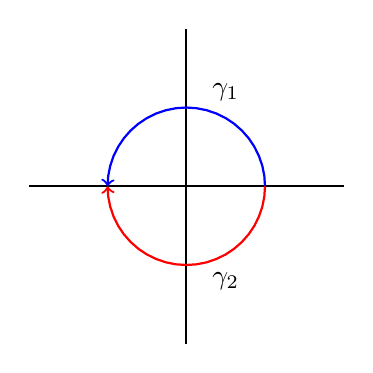
\begin{tikzpicture}
%\draw [help lines,black!20!white] (-1,-1) grid (4,4);

\draw[thick] (0,-2) -- (0,2);
\draw[thick] (-2,0) -- (2,0);

\draw [blue,thick,domain= 0:180, ->] plot ({cos(\x)}, {sin(\x)});
\draw [red,thick,domain= 180:360, <-] plot ({cos(\x)}, {sin(\x)});
\draw (0.5,-1.2) node {$\gamma_2$};
\draw (0.5,1.2) node {$\gamma_1$};

\end{tikzpicture}
\end{center}

The curve $\gamma_1$ is the upper semicircle of radius $1$ centered at $0$, travelled from $1$ to $-1$. We can parametrize it as $\gamma_1(t) = e^{it}$ for $t\in[0,\pi]$. Its derivative is $\gamma_1'(t) = ie^{it}$. So we compute the integral:
$$\int_{\gamma_1}\frac{1}{z}dz = \int_{0}^\pi \frac{1}{e^{it}}ie^{it}dt = \int_0^\pi idt = i\pi$$


The curve $\gamma_2$ is the lower semicircle of radius $1$ centered at $0$, travelled from $1$ to $-1$. We can parametrize it as $\gamma_2(t) = e^{-it}$ for $t\in[0,\pi]$. Its derivative is $\gamma_2'(t) = -ie^{it}$. So we compute the integral:
$$\int_{\gamma_2}\frac{1}{z}dz = \int_{0}^\pi -\frac{1}{e^{-it}}ie^{-it}dt = \int_0^\pi -idt = -i\pi$$

We find that $-i\pi = F(-1) = i\pi$, which tells us that $F$ isn't a function!
\end{ex}

In this example, we ran afoul of something very unfortunate: complex line integration is not path independent in general.

\subsection{Path Independence}

\begin{defbo}{Path Independence}{}\index{Path Independence}\index{Line Integral!path independent}
	Let $U\subset \C$ and $f:U\rightarrow \C$. $f$ has path independent line integrals in $U$ if $\int_{\gamma_1} fdz = \int_{\gamma_2}fdz$ for any curves $\gamma_1,\gamma_2$ in $U$ with the same start and end points.
\end{defbo}


When can we guarantee that $\int_{\gamma_1}f(z)dz = \int_{\gamma_2}f(z)dz$? To begin, let's investiage this equation a bit more. If these integrals are equal, then we can rearrange to get:

\begin{align*}0 &= \int_{\gamma_1} f(z)dz - \int_{\gamma_2}f(z)dz\\
&= \int_{\gamma_1} f(z)dz + \int_{-\gamma_2} f(z)dz \hspace{50pt} \text{From week 5 homework, Q6}\\
&= \int_{\gamma_1 + (-\gamma_2)}f(z)dz \hspace{95pt}\text{From week 5 homework, Q7}
\end{align*}

So, the integrals $\int_{\gamma_1}f(z)dz$ and $\int_{\gamma_2}f(z)dz$ are equal if and only if the integral $\int_{\gamma_1 - \gamma_2}f(z)dz$, over the closed curve $\gamma_1 + (-\gamma_2)$ is $0$. This looks an awful lot like a Cauchy Integral Theorem type result. However, we have no guarantees that $\gamma_1 + (-\gamma_2)$ is smooth or simple. We only know that it is piecewise smooth and closed.

So, for the moment, let's try to generalize the Cauchy-Integral theorem to handle piecewise smooth, closed curves. To do so, we need to overcome several hurdles. We need to:

\begin{itemize}
\item define integration over piecewise smooth curves
\item show we can generalize CIT to handle piecewise smooth curves
\item show we can generalize CIT to handle non-simple closed curves
\end{itemize}

So, to begin, we define:

\begin{defbo}{}{}\index{Integral!piecewise smooth curve}Let $\gamma$ be a piecewise smooth curve. Then $\gamma$ can be written as $\gamma = \gamma_1 + \gamma_2 + \dots + \gamma_n$, where each $\gamma_j$ is a smooth curve.

We define the integral $\int_{\gamma}f(z)dz$ as:
$$\int_{\gamma}f(z)dz = \sum_{j = 1}^n \int_{\gamma_j}f(z)dz$$
\end{defbo}

Now, fortunately, extending CIT to work over piecewise smooth curves takes no work. Green's theorem applies to piecewise smooth, simple, closed curves as well.

To handle the closed case, the idea is fairly simple. If we have a closed curve, such as:

\begin{center}
\begin{tikzpicture}
\draw[fill = lightgray] (0,0) to[out = 0, in = 270] (1,1) to[out = 90, in = 45] (0,0);
\draw[fill = DEFinner] (-1,0.4) to [out = 0, in = 225] (0,0) to[out = 225, in = 260] (-1,0.4);
\draw[fill = CORinner] (-1.5,-2) to[out =70 , in = 240] (-1,0.4) to[out = 100, in = 30] (-2,-1) to[out = 30, in = 70] (-1.5,-2);

\end{tikzpicture}
\end{center}

\noin which is composed of three different piecewise smooth, closed curves. If $f$ is analytic on a domain containing each of these curves and their insides, then we can use CIT on each of them. Then the total integral will be the sum of each of these integrals, which will be $0$.

A complete proof of this is much more technical. So our proof will be somewhat "hand-wavey".

\begin{thmbo}{Cauchy's Integral Theorem (version 2)}{CIT2}\index{Cauchy's Integral Theorem!version 2} Let $f$ be a function that is analytic on a domain $D$. Suppose that $\gamma$ is a closed, piecewise smooth curve such that $D$ contains $\gamma$ and all of the regions bounded by $\gamma$. Then:
$$\int_{\gamma}f(z)dz = 0$$
\end{thmbo}

Note that we have dropped the requirement that $f$ has continuous partials. We will continue to do this for the rest of the results in this chapter. This introduces a small hole for us. However, we can fix that by extending Cauchy-Goursat to piecewise smooth, simple, closed curves. Doing this is a bit technical however, so we will leave it for now.

\begin{proof}[Informal Proof:] The conditions on $\gamma$ ensure that $\gamma$ can be decomposed into:

\begin{itemize} 
\item countably many piecewise smooth, simple closed curves
\item countably many curves $\sigma_j$ such that $\gamma$ traverses each $\sigma_j$ an equal number in both directions
\end{itemize}

As such, we have that:

\begin{align*}\int_{\gamma}f(z)dz =& \sum_{\gamma_j \text{ is a simple, closed summand of} \gamma} \int_{\gamma_j}f(z)dz \\&+ \sum_{\sigma_j \text{ is a curve such that $\gamma$ traverses $\sigma_j$ an equal number of times in each direction}} n\left(\int_{\sigma_j} f(z)dz + \int_{-\sigma_j}f(z)dz\right)
\end{align*}

By our original CIT, the first summand is $0$. And since $\int_{\sigma_j}f(z)dz + \int_{-\sigma_j}f(z)dz = 0$, the second summand is $0$. Therefore:
$$\int_{\gamma}f(z)dz = 0$$

\end{proof}

We can use this to give one condition on path independence:

\begin{thmbo}{}{pathind} Suppose $f(z)$ is analytic with continuous partial derivatives on a domain $D$ containing the two curves $\gamma_1,\gamma_2$, which start and end at the same point, and which contains all points bounded between $\gamma_1,\gamma_2$. Then:
$$\int_{\gamma_1}f(z)dz = \int_{\gamma_2}f(z)dz$$
\end{thmbo}

\begin{proof} By CIT version 2:
$$\int_{\gamma_1 - \gamma_2}f(z)dz = 0$$

We showed earlier that this is equivalent to $\int_{\gamma_1}f(z)dz  =\int_{\gamma_2}f(z)dz$.
\end{proof}

The conditions on the curves in our CIT version 2 and in theorem \ref{thm:pathind} -- namely that the domain contains all regions bounded by the curve -- are generally annoying to handle on a case by case basis. And if we want our strategy to find a primitive to work, we need these conditions to hold for all curves from $z_0$ to $z$ in $D$. So we should expect this to require a condition on $D$. Fortunately, there's a nice topological condition we can impose that guarantees everything we need.

\begin{defbo}{Simply Connected Domains}{}\index{Domain!simply connected}

A domain $D$ is called simply connected if for every simple, closed curve $\gamma$ in $D$, that $\mathrm{in}(\gamma) \subset D$.

\end{defbo}

Intuitively, this means that the set has no "holes". For example:

\begin{ex}{}{} These domains are not simply connected because they have "holes":

\begin{center}
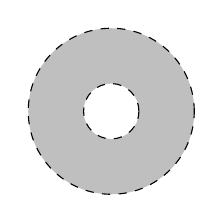
\begin{tikzpicture}[baseline=(current bounding box.center)]

\draw[fill = lightgray, dashed] (0,0) circle (30pt);
\draw[dashed, fill = white] (0,0) circle (10pt);

\end{tikzpicture}
\qquad or \qquad
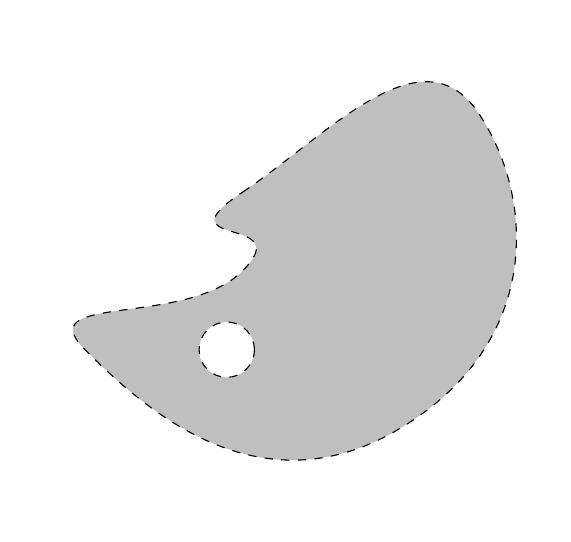
\begin{tikzpicture}[baseline=(current bounding box.center)]


\draw[dashed, fill = lightgray] plot [smooth cycle, tension = 1.3] coordinates {(0,0)  (0,1) (3,2) (2,-2) (-2,-1)};
\draw[dashed, fill = white] (-0.2,-1) circle (10pt);
\end{tikzpicture}

\end{center}

On the other hand, there are plenty of sets we're used to that are simply connected. $\C$, $\C\setminus (-\infty,0]$, and any open ball are all simply connected.
\end{ex}

This condition lets us state another version of the Cauchy Integral Theorem:

\begin{thmbo}{Cauchy's Integral Theorem (version 3)}{cit3}\index{Cauchy's Integral Theorem!version 3} Suppose $f(z)$ is analytic on a simply connected domain $D$. If $\gamma$ is any piecewise smooth, closed curve in $D$, then:

$$\int_{\gamma}f(z)dz = 0$$
\end{thmbo}

\begin{proof} This follows immediately from CIT version 2, since any closed curve in a simply connected domain satisfies the hypotheses of CIT version 2.\end{proof}

Having a sufficiently general version of the Cauchy Integral Theorem is a key step towards proving results about primitives. However, before we do that, we need another result. As it turns out, the result guaranteeing primitives that I would like to prove hinges on the ability to estimate integrals. So, before we can finish talking about primitives, we need the following result:

\begin{thmbo}{M-L Estimation of Integrals}{mlest}\index{M-L estimate} Suppose $\gamma:[a,b]\rightarrow \C$ is a piecewise smooth curve and $f(z)$ is a continuous function whose domain includes $\gamma$. Let $M = \max\left\{|f(\gamma(t))|\middle|t\in[a,b]\right\}$, and $L = \mathrm{Length}(\gamma)$. Then:
$$\left|\int_{\gamma}f(z)dz\right| \le ML$$
\end{thmbo}

\begin{proof} To begin, we will need to prove a nice fact: for any curve $g:[a,b]\rightarrow \C$, we have:
$$\left|\int_a^b g(t)dt\right| \le \int_a^b|g(t)|dt$$

Let $\int_a^bg(t)dt = re^{i\theta}$. Set $h(t) = e^{-i\theta}g(t)$. Then:
$$\int_a^bh(t)dt = \int_a^b e^{-i\theta}g(t)dt = e^{-i\theta}\int_a^bg(t)dt = r$$

So $\int_a^bh(t)dt \in \R$. We therefore have that $\RE\int_a^bh(t)dt = \int_a^b\RE(h(t))dt$. So, we have:

\begin{align*}\left|\int_a^bg(t)dt\right| &= r\\
&= \left|\int_a^b h(t)dt\right|\\
&= \left|\int_a^b \RE(h(t))dt\right|\\
&\le \int_a^b \left|\RE(h(t))\right|dt \hspace{30pt} (\text{from multivariable calc})\\
&\le \int_a^b |h(t)|dt \hspace{55pt} (\text{since }|\RE(h(t))| \le |h(t)|)\\
&= \int_a^b |g(t)|dt \hspace{55pt} (\text{since } |h(t)| = |e^{-i\theta}||g(t)| = |g(t)|)
\end{align*}


With this in hand, we can now proceed to prove the result we desire:

\begin{align*} \left|\int_{\gamma} f(z)dz\right| &= \left|\int_a^b f(\gamma(t))\gamma'(t)dt\right|\\
&\le \int_a^b |f(\gamma(t))||\gamma'(t)|dt\\
&\le \int_a^b M|\gamma'(t)|dt\\
&= M\int_a^b |\gamma'(t)|dt
\end{align*}

However, we know that $\int_a^b |\gamma'(t)|dt = L$, and so we have the desired inequality.
\end{proof}

This result is, for now, theoretically interesting. However, much later on in the course, it will become very useful in practice.

Now that we have a better Cauchy's Integral Theorem and this technical result, we can prove:

\begin{thmbo}{}{prims} If $f(z)$ is analytic on a simply connected domain $D$, then $f$ has a primitive on this domain.
\end{thmbo}

\begin{proof} Fix a point $z_0$ in $D$. For any point $z\in D$, we define
$$F(z) = \int_{\gamma_z}f(w)dw$$

\noin where $\gamma_z$ is any piecewise smooth curve from $z_0$ to $z$. By CIT version 3, we know that integration of $f$ in $D$ is path independent, so this function is well defined.

All that remains is to show that $F'(z) = f(z)$. To do this, we will show that $\ds\lim_{h\rightarrow 0} \left|\frac{F(z+h) - F(z) - hf(z)}{h}\right| = 0$, since this implies that $\ds\lim_{h\rightarrow 0} \frac{F(z+h) - F(z)}{h} = f(z)$. 


Let $\gamma_z$ be any curve from $z_0$ to $z$. Since $D$ is a domain, there exists a radius $r > 0$ such that $B_r(z) \subset D$, so we assume that $|h| < r$. Let $\gamma_h$ be the straight line from $z$ to $z+h$ given by $\gamma(t) = z+th$, $t\in[0,1]$. Notice that $\gamma_h \subset B_r(z)$, and that $\gamma_z+\gamma_h$ is a curve from $z_0$ to $z + h$ in $D$. As such $F(z+h) = \int_{\gamma_{z+h}} f(w)dw = \int_{\gamma_z} f(w)dw + \int_{\gamma_h}f(w)dw$. Therefore:


\begin{align*} =\lim_{h\rightarrow 0} \left|\frac{F(z+h) - F(z) - hf(z)}{h}\right|  &= \lim_{h\rightarrow 0} \left|\frac{1}{h} \int_{\gamma_h} f(w)dw - f(z)\right|\\
&=\lim_{h\rightarrow 0} \left|\frac{1}{h} \int_{\gamma_h} f(w)dw - \frac{1}{h}\int_{\gamma_h}f(z)dw\right|\\
&= \lim_{h\rightarrow 0} \left|\frac{1}{h}\int_{\gamma_h} (f(w) - f(z))dw\right|
\end{align*}

Now, since $f$ is continuous on $D$, then for any $\varepsilon > 0$ there exists $r > 0$ such that if $|w| < r$, then $|f(w) - f(z)|<\varepsilon$. If $|h| < r$, then for any $w$ on $\gamma_h$, we also have $|w| < r$. This gives us that $M = \max\{|f(w)|:w= \gamma_h(t)\} < \varepsilon$. Notice also that $\gamma_h$ has length $|h|$. So by M-L estimation, we have:

$$\lim_{h\rightarrow 0} \left|\frac{F(z+h) - F(z) - hf(z)}{h}\right| \le \lim_{h\rightarrow 0} \left| \frac{1}{h}\varepsilon |h|\right|  = \lim_{h\rightarrow 0} \frac{|h|}{|h|}\varepsilon = \varepsilon$$

Therefore, for any $\varepsilon > 0$, $0\le \lim_{h\rightarrow 0} \left|\frac{F(z+h) - F(z) - hf(z)}{h}\right| < \varepsilon$. So $\lim_{h\rightarrow 0} \left|\frac{F(z+h) - F(z) - hf(z)}{h}\right| = 0$ and $F'(z) = f(z)$.
\end{proof}

Alright, so this is fairly technical. However, it tells us that a lot of functions have primitives. However, note that this is only one direction. This does not say that if the domain isn't simply connected, then $f$ has no primitive.

\begin{ex}{}{} We know that $\frac{d\frac{1}{z}}{d\,z} = -\frac{1}{z^2}$. So, even though $\C\setminus\{0\}$ is not simply connected, $\frac{1}{z^2}$ has a primitive!

On the other hand, this does tell us that some fairly fantastical functions have primitives. For example, $\sin(\sin(\sin(e^{z\cos(z)})+z^2))\cos(z^3 - 1)$ has a primitive on $\C$! Good luck finding it, but it's there.
\end{ex}

Alright, so we have a result that tells us when a function has a primitive. Can we figure out when a function doesn't have a primitive? Well, remember that if $f$ has a primitive on $D$, then the integral of $f$ over any closed curve is automatically $0$, by $\C$FTC. This turns out to actually be an if and only if:

\begin{thmbo}{}{} Let $f$ be analytic on a domain $D$. Then $f$ has a primitive on $D$ if and only if $\int_\gamma f(z)dz = 0$ for any piecewise smooth, closed curve in $D$.\end{thmbo}

\begin{proof} If $f$ has a primitive, $\C$FTC gives that $\int_{\gamma}f(z)dz = 0$.

On the other hand, if $\int_{\gamma}f(z)dz =0$ for {\it every} $\gamma$, then our argument in simply connected case still applies. The integral definition of $F(z)$ is still well-defined. The rest of the argument doesn't use that $D$ is simply connected, and so the rest of the proof still applies!\end{proof}

In practice, we can use this to conclude when something doesn't have a primitive on a domain.

\begin{ex}{}{} $f(z) = \frac{1}{z}$ does not have a primitive on any domain containing the unit circle. To prove this, note that we have shown that the integral of $f(z)$ from $1$ to $-1$ over the upper unit circle is $i\pi$, while over the lower unit circle we have $-i\pi$. All together, this tells us that the integral of $f(z)$ over the whole unit circle is $2\pi i$.

Since there is a closed curve $\gamma$ in $D$ with $\int_{\gamma}f(z)dz \ne 0$, we cannot have a primitive.
\end{ex}

\section{A Roadmap}

So far, we have seen how to handle a large class of integrals. integrating analytic functions on simply connected domains is easy. How do we handle the case where we want to integrate over a domain which is not simply connected? For example, how do we find:
$$\int_{|z| = 2} \frac{1}{z^4 + 1}dz \qquad \text{or} \qquad \int_{|z| = 1}e^{\frac{1}{z}}dz$$

The first of these functions is analytic on $\C\setminus\{\pm\frac{1+i}{\sqrt{2}},\pm \frac{1-i}{\sqrt{2}}\}$, and the second is analytic on $\C\setminus\{0\}$. Neither of their domains contains the inside of the circles. So we cannot apply the Cauchy Integral Theorem.

Is there a unifying theory that will tells us how to handle integrals like this? It turns out there is. It hinges around the notion of an ``isolated singularity".

\begin{defbo}{}{}\index{Isolated Singularity}An {\bf isolated singularity} $z_0\in\C$ of a function $f$ is a point such that:

\begin{itemize} 
	\item $f$ is discontinuous at $z_0$ or $f$ is not defined at $z_0$
	\item $f$ is analytic on $B_r(z_0)\setminus\{z_0\}$ for some $r > 0$
\end{itemize}
\end{defbo}

So, an isolated singularity is a point where the function is not continuous, but is analytic around it.

\begin{ex}{}{} $\frac{1}{z}$ has an isolated singularity at $z = 0$.

$\frac{1}{z^4 - 1}$ has isolated singularities at $z= \pm 1,\pm i$.

$\Log(z)$ has no isolated singularities.
\end{ex}

The strategy for integrating on curves whose inside contains isolated singularity depends on the type of singularity. There are three types: removable discontinuities, poles, and essential singularities.

\begin{ex}{}{} $\frac{z^2 -1}{z - 1}$ has a removable discontinuity at $z = 1$. $\frac{\sin(z)}{z}$ has a removable discontinuity at $z = 0$.\end{ex}

\begin{defbo}{Removable Discontinuity}{}\index{Removable Discontinuity}\index{Isolated Singularity!removable discontinuity} A {\bf removable discontinuity} $z_0$ is an isolated singularity such that:

$$\lim_{z\rightarrow z_0} f(z)\text{ exists}$$
\end{defbo}

So, a removable discontinuity is a an isolated singularity which can be filled. It turns out that filling this discontinuity results in an analytic function, and so the Cauchy Integral Theorem still applies in this case!

\begin{defbo}{Pole of order $n$}{pole}\index{Pole}\index{Isolated Singularity!pole}\index{Simple Pole}\index{Pole!simple} A {\bf pole of order $n$} is an isolated singularity $z_0$ such that there exists a function $g(z)$ which is analytic on $B_r(z_0)$, $g(z_0)\ne 0$, and:

$$f(z) = \frac{g(z)}{(z-z_0)^n}$$

A pole of order $1$ is called a {\bf simple pole}.
\end{defbo}

These isolated singularities behave like vertical asymptotes. We will see later on that $\lim_{z\rightarrow z_0}f(z) = \infty$, and the order tells you how quickly the function tends to $\infty$.

\begin{ex}{}{}$\frac{1}{z^4 - 1}$ has simple poles at each of $\pm1, \pm i$. For example, at $z = 1$, we can write $g(z) = \frac{1}{(z+1)(z^2 + 1)}$ and $\frac{1}{z^4 - 1} = \frac{g(z)}{z-1}$. The function $g(z)$ is analytic on $\C\setminus \{-1,i,-i\}$, and so in particular it is analytic on $B_1(1)$.
\end{ex}

Lastly, we have the worst behaved of the lot.

\begin{defbo}{Essential Singularity}{}\index{Essential Singularity}\index{Isolated Singularity!essential Singularity} An {\bf essential singularity} is an isolated singularity that is neither a pole nor removable.\end{defbo}

It turns out that this type of singularity behaves terribly. Not only does $\lim_{z\rightarrow z_0}f(z)$ not exist, it's also not $\infty$. Furthermore, it turns out that for any $r > 0$, $\{f(w)|w\in B_r(z_0)\setminus\{z_0\}\} = \C$ or $\C\setminus\{0\}$. This result, which we won't prove, is called the Great Picard's Theorem. So, $f(z)$ takes on every value (except maybe one value) infinitely often near its essential singularities. This is incredibly bad behavior. This is akin to a function like $\frac{\sin\left(\frac{1}{x}\right)}{x}$ on $\R$.

For each of these types of isolated singularity, we're going to have a particular method:

\begin{itemize} \item To integrate around removable discontinuities, we will soon see that the Cauchy Integral Theorem is sufficient.
\item To integrate around a pole, we will need to talk about the Cauchy Integral Formula.
\item To integrate around essential singularities, we are going to need to talk about power series and Laurent series. This will lead us to a nice result, called the Residue theorem, which will encapsulate each of these methods.
\end{itemize}

\section{Integrating Around Poles}

Our first stop along this roadmap are functions with poles. How do we integrate $\int_\gamma f(z)dz$ if $f(z)$ has poles inside $\gamma$? In particular, we're going to discuss simple poles first. For example, how do we find:
$$\int_{|z| = 1} \frac{e^z}{z}dz$$

Since this function isn't analytic inside the curve, the Cauchy Integral Theorem does not apply. We have no reasonable guess as to a primitive (and indeed, this function does not have a primitive on any domain containing the unit circle!). What if we try using the definition of the integral?

\begin{ex}{}{} Let $\gamma(t) = e^{it}$ for $t\in [0,2\pi]$. Then:

$$\int_{\gamma} \frac{e^z}{z}dz = \int_0^{2\pi} \frac{e^{e^{it}}}{e^{it}}ie^{it}dt = i\int_0^{2\pi} e^{\cos(t)}(\cos(\sin(t)) + i\sin(\sin(t)))dt$$

How exactly are we supposed to evaluate this mess of an integral? It doesn't appear likely that any of the techniques from first year calculus will be of much use here.\end{ex}

So, none of our techniques so far work. We need something new. It turns out there is a general theorem that will let us handle any function with a simple pole.


\subsection{Cauchy's Integral Formula}

The key result for integrating around poles is called Cauchy's integral formula.

\begin{thmbo}{Cauchy's Integral Formula}{CIF}\index{Cauchy's Integral Formula}
Suppose $f(z)$ is analytic on a domain $D$ such that $\{z\in\C||z-z_0|\le r\} \subset D$. Let $\gamma$ be the circle of radius $r$ centered at $z_0$, travelled once counterclockwise. Then:
$$\int_{\gamma} \frac{f(z)}{z - z_0}dz = 2\pi i f(z_0)$$
\end{thmbo}

Before we prove this, let's see how it applies to our previous example.

\begin{ex}{}{} Let $f(z) = e^z$. This is entire, so is analytic on $\C$. $\C$ is a domain containing $\{z\in\C||z-z_0|\le 1\}$. Let $|z| = 1$ refer to the unit circle travelled once counterclockwise. Then CIF applies to give:

$$\int_{|z| = 1}\frac{e^z}{z}dz = \int_{|z| = 1} \frac{f(z)}{z-0}dz = 2\pi i f(0) = 2\pi i e^0 = 2\pi i$$
\end{ex}

Notice: the theorem is very easy to apply. No complicated arithmetic involved. However, we do need to check the conditions of the theorem before we apply it. This takes some care.

Let's prove this theorem. The proof contains at least one very useful idea.

\begin{proof}Let $\gamma_s$ be the circle of radius $s$ centered at $z_0$, where $s\in(0,r]$. We may assume, without loss of generality, that each $\gamma_s$ starts at the angle $\theta = 0$ and ends at $\theta = 2\pi$. We define a function $F(s)$ as follows:

$$F(s) = \int_{\gamma_s}\frac{f(z)}{z-z_0}dz$$

So the integral we are interested in is $F(r)$. We shall prove two facts about $F(s)$:

\begin{itemize}
\item $F(s)$ is constant on $(0,r]$.
\item $\lim_{s\rightarrow 0^+} F(s) = 2\pi i f(z_0)$.
\end{itemize}

To prove that $F(s)$ is constant, consider the following picture:

\begin{center}
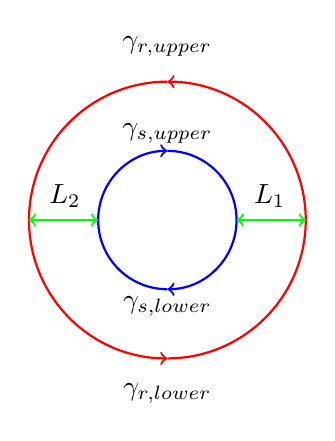
\begin{tikzpicture}

\draw[red, ->, thick] ([shift = (90:50pt)] 0,0) arc (90:270:50pt);
\draw[red, ->, thick] ([shift = (270:50pt)] 0,0) arc (270:450:50pt);
\draw[blue, <-, thick] ([shift = (-90:25pt)] 0,0) arc (-90:90:25pt);
\draw[blue, <-, thick] ([shift = (90:25pt)] 0,0) arc (90:270:25pt);

\draw[green, <->, thick] (0.88,0) -- (1.76,0);
\draw[green, <->, thick] (-0.88,0) -- (-1.76,0);

\draw (0,2.2) node {$\gamma_{r,upper}$};
\draw (0,-2.2) node {$\gamma_{r,lower}$};

\draw (0, 1.1) node {$\gamma_{s,upper}$};
\draw (0, -1.1) node {$\gamma_{s,lower}$};

\draw (1.3,0.3) node {$L_1$};
\draw (-1.3,0.3) node {$L_2$};
\end{tikzpicture}
\end{center}

\noin where $L_1$ and $L_2$ travel from left to right.

Notice that $-\gamma_s = \gamma_{s,upper} + \gamma_{s,lower}$ (since $\gamma_{s,upper}$ and $\gamma_{s,lower}$ are travelling clockwise) and that $\gamma_r = \gamma_{r,upper} + \gamma_{r,lower}$.

Now, we know that $\frac{f(z)}{z-z_0}$ is analytic on $D\setminus \{z_0\}$, which is a domain containing the closed curve $\gamma_{r,upper} + L_2 + \gamma_{s,upper} + L_1$. So by CIT:
$$\int_{\gamma_{r,upper} + L_2 + \gamma_{s,upper} + L_1} \frac{f(z)}{z-z_0}dz = 0$$

And similarly:
$$\int_{\gamma_{r,lower} - L_1 + \gamma_{s,lower} - L_2} \frac{f(z)}{z-z_0}dz = 0$$

Adding these two together gives us that:

\begin{align*}&\int_{\gamma_{r,upper}} \frac{f(z)}{z-z_0} dz + \int_{L_2} \frac{f(z)}{z-z_0} dz + \int_{\gamma_{r,lower}} \frac{f(z)}{z-z_0} dz + \int_{L_1} \frac{f(z)}{z-z_0} dz \\
&+\int_{\gamma_{s,upper}} \frac{f(z)}{z-z_0} dz + \int_{-L_1} \frac{f(z)}{z-z_0} dz + \int_{\gamma_{s,lower}} \frac{f(z)}{z-z_0} dz + \int_{-L_2} \frac{f(z)}{z-z_0} dz  = 0\end{align*}

After simplifying, we find that:

$$\int_{\gamma_{r}} \frac{f(z)}{z-z_0} dz + \int_{-\gamma_{s}} \frac{f(z)}{z-z_0}dz = 0$$

As such, $F(s) = F(r)$ for all $s \in (0,r)$. So $F$ is constant on $(0,r]$.

So, we see that $\lim_{s\rightarrow 0^+} F(s) = \lim_{s\rightarrow 0^+}F(r) = F(r)$.

All that remains is for us to actually compute this limit. To do that, we go to the definition of the integral.

$$\int_{\gamma_s} \frac{f(z)}{z-z_0}dz = \int_0^{2\pi} \frac{f(z_0 + se^{it})}{se^{it}}ise^{it}dt = \int_0^{2\pi} if(z_0 + se^{it})dt$$

We claim that $\lim{s\rightarrow 0^+} \int_0^{2\pi} if(z_0 + se^{it})dt =2\pi i f(z_0)$. Consider the difference:

\begin{align*}\lim_{s\rightarrow 0^+} \left|\int_0^{2\pi} if(z_0 + se^{it})dt - 2\pi i f(z_0)\right| &= \lim_{s\rightarrow 0^+} \left|\int_0^{2\pi} if(z_0 + se^{it})dt - \int_0^{2\pi} if(z_0)dt\right|\\
&\le \lim_{s\rightarrow 0^+} \int_0^{2\pi} |f(z_0 + se^{it}) - f(z_0)|dt\\
&\le \lim_{s\rightarrow 0^+} 2\pi \max\{|f(w) - f(z_0)|| w\in \{z\in\C||z-z_0|\le s\}\}
\end{align*}

Now, since $f$ is continuous at $z_0$, we see that  $\lim_{s\rightarrow 0^+}\max\{|f(w) - f(z_0)|| w\in \{z\in\C||z-z_0|\le s\}\} = 0$. So the squeeze theorem gives us that:
$$\lim_{s\rightarrow 0^+} \left|\int_0^{2\pi} if(z_0 + se^{it})dt - 2\pi i f(z_0)\right| = 0$$

As such, $\lim_{s\rightarrow 0^+} \int_0^{2\pi} if(z_0 + se^{it})dt =2\pi i f(z_0)$ as desired.

Putting it all together, we get that:

$$\int_{\gamma_r} \frac{f(z)}{z-z_0}dz = F(r) = \lim_{s\rightarrow 0^+} F(s) = 2\pi i f(z_0)$$

\end{proof}

While technical, this proof has a really important idea. The technique for showing that the integrals over the two circles are equal is fairly useful. For example:

\begin{ex}{}{}Let $\gamma$ be the circle of radius $3$ centered at $0$, travelled once counterclockwise. Find $\int_{\gamma} \frac{1}{z-1}dz$.

As written, CIF doesn't apply. This first version of CIF only applies to circles centered at $z_0$, which in this case is $1$.

However, our technique from the proof of CIF gives that:

$$\int_{\gamma} \frac{1}{z-1}dz = \int_{|z-1|=1} \frac{1}{z-1}dz$$

And now we're in a situation where CIF applies. It gives $\int_{\gamma} \frac{1}{z-1}dz = 2\pi i$.\end{ex}

We continue with another example of how to use the Cauchy Integral Formula:

\begin{ex}{}{} Let $\gamma$ be the circle of radius $2$ centered at $0$, travelled once counterclockwise. Find $\int_{\gamma} \frac{1}{z^2 + 1}dz$.

The function $\frac{1}{z^2 + 1} = \frac{1}{(z+i)(z-i)}$ has two simple poles inside the curve. So CIF doesn't immediately apply. Instead, we need to turn this into a situation where it does. Consider the following curves:


\begin{center}
\begin{tikzpicture}[baseline=(current bounding box.center)]

\draw [help lines,black!20!white] (-3,-3) grid (3,3);

\draw[red, thick, decoration={markings, mark=at position 0.5 with {\arrow{>}}},
		postaction = {decorate}] 
	([shift = (-85:56pt)] 0,0) arc (-85:85:56pt);
\draw[red, thick, decoration={markings, mark=at position 0.5 with {\arrow{>}}},
		postaction = {decorate}] 
	([shift = (95:56pt)] 0,0) arc (95:265:56pt);
	
	
	
	
\draw[blue, thick, decoration={markings, mark=at position 0.5 with {\arrow{<}}},
		postaction = {decorate}] 
	([shift = (105:20pt)] 0,1) arc (105:435:20pt);

\draw[blue, thick, decoration={markings, mark=at position 0.5 with {\arrow{<}}},
		postaction = {decorate}] 
	([shift = (-75:20pt)] 0,-1) arc (-75:255:20pt);

\draw[fill = black] (0,1) circle (2pt) node[above] {$i$};
\draw[fill = black] (0,-1) circle (2pt)node[above] {$-i$};


\draw[green, thick, decoration={markings, mark=at position 0.6 with {\arrow{>}}},
		postaction = {decorate}] 
	(0.165,1.97) -- (0.165,1.67);

\draw[green, thick, decoration={markings, mark=at position 0.6 with {\arrow{<}}},
		postaction = {decorate}] 
	(-0.165,1.97) -- (-0.165,1.67);

\draw[black, thick, decoration={markings, mark=at position 0.6 with {\arrow{<}}},
		postaction = {decorate}] 
	(0.165,-1.97) -- (0.165,-1.67);

\draw[black, thick, decoration={markings, mark=at position 0.6 with {\arrow{>}}},
		postaction = {decorate}] 
	(-0.165,-1.97) -- (-0.165,-1.67);

\draw (2,0) node[right]{$\gamma_1$};

\end{tikzpicture}
\qquad and \qquad
\begin{tikzpicture}[baseline=(current bounding box.center)]

\draw [help lines,black!20!white] (-3,-3) grid (3,3);

\draw[red, thick, decoration={markings, mark=at position 0.7 with {\arrow{>}}},
		postaction = {decorate}] 
	([shift = (85:56pt)] 0,0) arc (85:95:56pt);
\draw[red, thick, decoration={markings, mark=at position 0.7 with {\arrow{>}}},
		postaction = {decorate}] 
	([shift = (265:56pt)] 0,0) arc (265:275:56pt);
	
	
	
	
\draw[blue, thick, decoration={markings, mark=at position 0.7 with {\arrow{>}}},
		postaction = {decorate}] 
	([shift = (105:20pt)] 0,1) arc (105:75:20pt);

\draw[blue, thick, decoration={markings, mark=at position 0.7 with {\arrow{>}}},
		postaction = {decorate}] 
	([shift = (285:20pt)] 0,-1) arc (285:255:20pt);




\draw[green, thick, decoration={markings, mark=at position 0.7 with {\arrow{<}}},
		postaction = {decorate}] 
	(0.165,1.97) -- (0.165,1.67);

\draw[green, thick, decoration={markings, mark=at position 0.7 with {\arrow{>}}},
		postaction = {decorate}] 
	(-0.165,1.97) -- (-0.165,1.67);

\draw[black, thick, decoration={markings, mark=at position 0.7 with {\arrow{>}}},
		postaction = {decorate}] 
	(0.165,-1.97) -- (0.165,-1.67);

\draw[black, thick, decoration={markings, mark=at position 0.7 with {\arrow{<}}},
		postaction = {decorate}] 
	(-0.165,-1.97) -- (-0.165,-1.67);

\draw (0,2) node[above]{$\gamma_2$};
\draw (0,-2) node[below]{$\gamma_3$};

\end{tikzpicture}
\end{center}

Since none of these three curves enclose $\pm i$, CIT applies to give that:
$$\int_{\gamma_j} \frac{1}{z^2+1}dz = 0$$

\noin for each $j = 1,2,3$. Adding them together gives that:

$$0 = \sum_{j=1}^3 \int_{\gamma_j} \frac{1}{z^2+1}dz = \int_{C} \frac{1}{z^2+1}dz - \int_{C_1} \frac{1}{z^2+1}dz - \int_{C_2} \frac{1}{z^2+1}dz $$

\noin where $C$ is the large circle travelled once counterclockwise, $C_1$ is the smaller circle around $i$ travelled once counterclockwise, and $C_2$ is the smaller circle around $-i$ travelled once counterclockwise. This second equality comes from noticing that the green lines in $\gamma_1$ and $\gamma_2$ are travelled in opposite directions, so their integrals cancel out. The same is true for the black lines in $\gamma_1$ and $\gamma_3$.

So we are left with the red arcs which together make $C$, and the blue arcs which together make $-C_1$ and $-C_2$ (notice that the blue arcs are travelling clockwise!)

All together, this shows that $\int_{C}\frac{1}{z^2 + 1}dz = \int_{C_1}\frac{1}{z^2 + 1}dz + \int_{C_1}\frac{1}{z^2 + 1}dz$. We now calculate these two integrals using CIF.

For the integral around $C_1$, let $f(z) = \frac{1}{z+i}$. Then $f(z)$ is analytic on $\C\setminus\{-i\}$, which is a domain containing $C_1$ and its inside. So:

$$\int_{C_1} \frac{1}{z^2+1} dz = \int_{C_1}\frac{f(z)}{z-i}dz = 2\pi i f(i) = \pi$$

And similarly, $\int_{C_2}\frac{1}{z^2 + 1}dz = -\pi$. So all together, $\int_C \frac{1}{z^2+1}dz = 0$.
\end{ex}

This example suggests a general technique.

\subsection{The Deformation Theorem}

We can mimic the above technique for domains containing more poles. This will let us break up some quite complicated integrals into a handful of integrals which can be handled by other techniques (for example, the CIF.)

\begin{thmbo}{The Deformation Theorem}{deform}\index{Deformation Theorem} Let $D$ be a domain and $z_1,\dots,z_n \in D$. Suppose $\gamma$ is a piecewise smooth, positively oriented, simple closed curve in $D$ such that the inside of $\gamma$ is in $D$ and each $z_j$ is inside $\gamma$. Suppose that $f(z)$ is analytic on at least $D\setminus\{z_1,\dots,z_n\}$. Further, suppose $r_1,\dots,r_n > 0$ satisfy that $\{z\in\C||z-z_j| \le r_j\}\subset D$. Let $C_j$ be the circle of radius $r_j$ centered at $z_j$ travelled once counterclockwise. Then:
$$\int_{\gamma} f(z)dz = \sum_{j=1}^n \int_{C_j} f(z)dz$$
\end{thmbo}

\begin{proof} We proceed by induction. Suppose $n = 1$. Fix $\theta \in (0,\pi)$. Consider the rays $R_+ = \{z_1 + re^{i\theta}|r \ge r_j\}$ and $R_- = \{z_1 + re^{-i\theta}|r \ge r_j\}$. We have something like the following picture:


\begin{center}
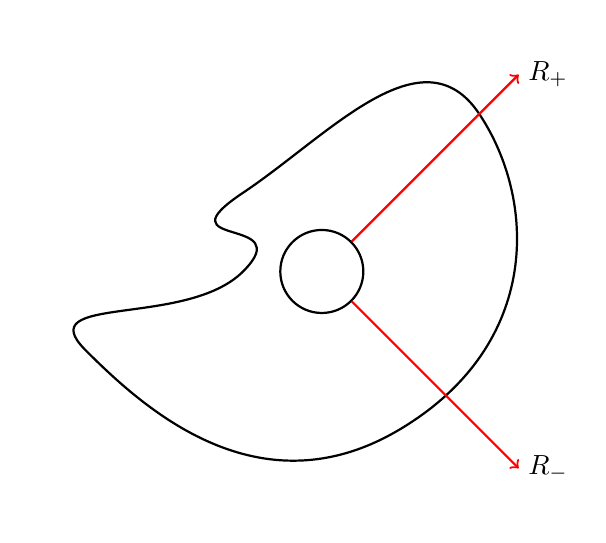
\begin{tikzpicture}

\draw[thick, ->] plot [smooth cycle, tension = 1.3] coordinates {(0,0)  (0,1) (3,2) (2,-2) (-2,-1)};
\draw[thick, <-] (1,0) circle (15pt);

\draw[thick, red,->] (1.38,0.38) -- (3.5,2.5);
\draw (3.5,2.5) node[right]{$R_+$};
\draw[thick, red,->] (1.38,-0.38) -- (3.5,-2.5);
\draw (3.5,-2.5) node[right]{$R_-$};
\end{tikzpicture}

\end{center}

Since $z_j$ is inside $\gamma$, there exists $r_+$ and $r_-$ which are the closest intersections of $R_+$ and $R_-$ with $\gamma$ to the point $z_j$. Let $L_+$ be the line segment from $z_0 + r_-e^{i\theta}$ to $z_0 + r_+e^{i\theta}$ and $L_-$ the line segment from $z_0 + r_je^{-i\theta}$ to $z_0 + r_-e^{-i\theta}$.

These intersections divide $\gamma$ into two segments: $\gamma_1$ and $\gamma_2$.  Specifcally, $\gamma_1$ starts at the intersection of $\gamma$ with $R_+$ and travels $\gamma$ in the positive orientation until it hits the intersection with $R_-$. And $\gamma_2$ starts where $\gamma$ intersects $R_-$ and travels along $\gamma$ until it hits $R_+$ 

Similarly, the circle is divided into two segments: the arc $A_1$ from the angle $-\theta$ to $\theta$, and the arc $A_2$ from the angle $\theta$ to $2\pi - \theta$.

By our construction and the assumption that $C_1$ is inside $\gamma$, $z_1$ is not inside either of $\gamma_1 - L_- - A_2 + L_+$ or $\gamma_2 - L_+ - A_1 + L_-$. (Follow the picture to see why these are the curves we want.) These are each simple closed, positively oriented curves whose insides are in $D\setminus\{z_1\}$. As such, CIT gives that:

$$\int_{\gamma_1 - L_- - A_2 + L_+} f(z)dz = \int_{\gamma_2 - L_+ - A_1 + L_-}f(z)dz = 0$$

Adding these together, we get that:

$$\int_{\gamma_1} f(z)dz - \int_{L_-}f(z)dz -\int_{A_2}f(z)dz + \int_{L_+}f(z)dz + \int_{\gamma_2} f(z)dz - \int_{L_+}f(z)dz - \int_{A_1}f(z)dz - \int_{L_1}f(z)dz = 0$$

Simplifying gives that $\int_{\gamma} f(z)dz - \int_{C_1}f(z)dz = 0$, as desired.

Proceeding with the induction, suppose the claim is true for $k$ points $z_1,\dots, z_k$ where $k\le n$.

Decompose $\gamma$ as in the case for $n = 1$. However, in this case, we will have that $\gamma_1 - L_- - A_2 + L_+$ will now have (without loss of generality) $z_2,\dots,z_k$ inside $\gamma_1 - L_- - A_2 + L_+$ for some $k\le n$. The remaining $z_{k+1},\dots,z_n$ (if there are any) will be inside $\gamma_2 - L_+ - A_1 + L_-$ necessarily. Since $\{z_2,\dots,z_k\}$ contains at most $n-1$ points, the induction hypothesis applies to give:

$$\int_{\gamma_1 - L_- - A_2 + L_+} f(z)dz = \sum_{j = 2}^k \int_{C_j} f(z)dz$$

\noin and similarly the induction hypothesis gives us that:

$$\int_{\gamma_2 - L_+ - A_1 + L_-} f(z)dz = \sum_{j = k+1}^n \int_{C_j} f(z)dz$$

Adding these two together, as in the $n=1$ case, gives:

$$\int_{\gamma} f(z)dz - \int_{C_1}f(z)dz = \sum_{j = 2}^n \int_{C_j}f(z)dz$$

Rearranging gives the desired result.
\end{proof}

As an easy consequence of this, we can state a more general version of the Cauchy Integral Formula:

\begin{corbo}{Cauchy's Integral Formula (vII)}{CIF2}\index{Cauchy's Integral Formula}
Suppose $f(z)$ is analytic on a domain $D$. Let $\gamma$ be a piecewise smooth, positively oriented, simple closed curve in $D$ whose inside is in $D$. Suppose $z_0$ is inside $\gamma$. Then:

$$\int_{\gamma} \frac{f(z)}{z-z_0}dz = 2\pi if(z_0)$$
\end{corbo}

This follows immediately from deforming $\gamma$ to a circle and using our original CIF.

\subsection{Poles of Higher Order - The Generalized Cauchy Integral Formula}

Now that we know how to integrate curves surrounding a simple pole, or multiple simple poles, how do we handle integrating around higher order poles? For example, how do we find $\int_{|z|=1}\frac{e^z}{z^2}dz$? It turns out that we can generalize the CIF to handle this.

\begin{thmbo}{The Generalized Cauchy Integral Formula (or the Cauchy Differentation Formula)}{GCIF}\index{Cauchy's Integral Formula!Generalized}\index{Cauchy's Differentiation Formula}
Suppose $f(z)$ is analytic on a domain $D$. Let $\gamma$ be a piecewise smooth, positively oriented, simple closed curve in $D$ whose inside is in $D$. Suppose $z_0$ is inside $\gamma$. Suppose $n > 0$. Then:

$$\int_{\gamma} \frac{f(z)}{(z-z_0)^n}dz = \frac{2\pi i}{(n-1)!}f^{(n-1)}(z_0)$$
\end{thmbo}

The key to proving this is a result from multivariable calculus called the Leibniz Integral Rule.

\begin{lem} Suppose $f(w,z)$ is continuous in both $z$ and $w$ on some region $R$ such that if $(w_0,\gamma(t)) \in R$ for all $t$ whenever there exists $(w_0,z)\in R$. Further, suppose that $f_w(w,z)$ is continuous in both $z$ and $w$. Then:

$$\frac{d}{dw} \int_{\gamma} f(w,z)dz = \int_{\gamma} \frac{\partial}{\partial w} f(w,z)dz$$
\end{lem}

We will not be proving this. We move on to the proof of our theorem:

\begin{proof} We proceed by induction. For $n = 1$, the claim holds by the regular Cauchy Integral Formula.

Suppose the claim holds for some $n$. Let $g(z_0,z) = \frac{f(z)}{(z-z_0)^n}$. Notice that since $z_0$ is inside $\gamma$ and $z$ is on $\gamma$, that $g(z_0,z)$ is continuous in $z_0$ and $z$ (we can actually take $z$ close to $\gamma$, since $z_0$ has some positive distance between it and $\gamma$). Further:

$$\frac{\partial}{\partial z_0} g(z_0,z) = \frac{nf(z)}{(z-z_0)^{n+1}}$$

\noin is also continuous on the same region, for the same reason. As such, Leibniz's rule gives:

\begin{align*}\int_{\gamma} \frac{f(z)}{(z-z_0)^{n+1}}dz &= \int_{\gamma} \frac{1}{n} \frac{\partial}{\partial z_0} g(z_0,z) dz\\
&= \frac{1}{n}\frac{d}{dz_0}\int_{\gamma} g(z_0,z)dz\\
&= \frac{1}{n} \frac{d}{dz_0}\int_{\gamma} \frac{f(z)}{(z-z_0)^n}dz
\end{align*}

However, our induction hypothesis gives that $\int_{\gamma} \frac{f(z)}{(z-z_0)^n}dz = \frac{2\pi i}{(n-1)!}f^{(n-1)}(z_0)$. So:

\begin{align*}\int_{\gamma} \frac{f(z)}{(z-z_0)^{n+1}}dz &= \frac{1}{n}\frac{d}{dz_0}\frac{2\pi i}{(n-1)!}f^{(n-1)}(z_0)\\
&= \frac{2\pi i}{n!}f^{(n)}(z_0)
\end{align*}

\end{proof}

Note that at no point did we assume that the derivatives $f^{(n)}(z_0)$ exist. In fact, the Leibniz rule gives us that they exist, since they're equal to these integrals which do exist! As a corollary:

\begin{corbo}{Holomorphic Functions are Smooth}{}
If $f$ is holomorphic on a domain $D$, then $f$ is infinitely differentiable (otherwise known as smooth) on $D$.
\end{corbo}

Let's finish off with an example of using the generalized CIF.

\begin{ex}{}{} Let $\gamma$ be the circle of radius $2$ centered at $0$ travelled twice clockwise. Find $\int_{\gamma} \frac{\sin(z)}{(z^2+1)^2}dz$.

This function has two double poles, $z = \pm i$. Let $C$ be the circle of radius $2$ centered at $0$ travelled once clockwise. Then:

$$\int_{\gamma} \frac{\sin(z)}{(z^2+1)^2}dz = -2\int_{C}\frac{\sin(z)}{(z^2+1)^2}dz$$

By the deformation theorem:

$$\int_{C} \frac{\sin(z)}{(z^2+1)^2} dz = \int_{|z-i|=1} \frac{\sin(z)}{(z^2+1)^2}dz + \int_{|z+i|=1} \frac{\sin(z)}{(z^2+1)^2}dz$$

For the circle centered at $i$, we let $f(z) = \frac{\sin(z)}{(z+i)^2}$. Then $\frac{\sin(z)}{(z^2+1)^2} = \frac{f(z)}{(z-i)^2}$. Since $f(z)$ is analytic on $\C\setminus\{-i\}$, we can apply the generalized CIF to get:

$$\int_{|z-i|=1} \frac{\sin(z)}{(z^2+1)^2} dz = 2\pi i f'(i)$$

Now, $f'(z) = \frac{\cos(z)(z+i)^2 - 2\sin(z)(z+i)}{(z+i)^4}$, so: 
$$f'(i) = \frac{\frac{e^{-1} + e}{2}(2i)^2 - 2\frac{e^{-1} - e}{2i}(2i)}{16} = \frac{-4(e^{-1} + e) - 4(e^{-1} - e)}{32} = -\frac{1}{4e}$$

And so $\int_{|z-i|=1}\frac{\sin(z)}{(z^2+1)^2}dz = -\frac{\pi i }{2e}$.

For the circle centered at $-i$, we follow the same procedure with $g(z) = \frac{\sin(z)}{(z-i)^2}$. We find that:

$$\int_{|z+i|=1} \frac{\sin(z)}{(z^2+1)^2}dz = 2\pi i g'(-i)$$

And we calculate:

$$g'(-i) = \frac{-4\cos(-i) + 4i\sin(-i)}{16} = -4\frac{e^{i*i}}{16} = -\frac{1}{4e}$$

As such, $\int_{|z+i|=1}\frac{\sin(z)}{(z^2+1)^2}dz = -\frac{\pi i }{2e}$.

All together, $\int_{\gamma} \frac{\sin(z)}{(z^2+1)^2}dz = -2(-\frac{\pi i }{2e} -\frac{\pi i }{2e}) = \frac{2\pi i }{e} $.
\end{ex}

\section{Liouville's Theorem}

For the moment, we take a small detour from our roadmap to investigate a peculiar property of entire functions. Entire functions behave quite differently than we're used to. For example, our intuition says that the function $f(z) = \sin(z)$ should be bounded. After all, for $x \in \mathbb{R}$, $-1 \le \sin(x) \le 1$. However, we've seen that $\sin(z)$ is not a bounded function!

This is an example of a much more general phenomenon:

\begin{thmbo}{Liouville's Theorem}{Lioville}\index{Liouville's Theorem} Every bounded, entire function is constant.\end{thmbo}
\begin{proof} ~
\paragraph{Proof idea:} To show $f(z)$ is constant, we can show that $f'(z) = 0$ for all $z \in \C$.

To connect $f'(z)$ to the fact that $f(z)$ is bounded, we go through Cauchy's integral formula, which connects $f'(z)$ to $f(z)$.

\paragraph{Proof:} 
Suppose $f(z)$ is bounded and entire, but is non-constant. Let $M \in \mathbb{R}$ such that $|f(z)| \le M$ for all $z\in \C$.

Let $\gamma_R$ be the circle of radius of circle $R$, centered at $a$, travelled once counter-clockwise. Since $f(z)$ is entire, Cauchy's integral formula tells us that:

$$2\pi i f'(a) = \int_{\gamma_R} \frac{f(z)}{(z-a)^2}dz$$

We would like to show this integral is $0$. However, we don't have any way to calculate it. Instead, let's estimate:

$$|2\pi i f'(a)| = \left| \int_{\gamma_R} \frac{f(z)}{(z-a)^2}dz\right| \le \int_{\gamma_R} \left|\frac{f(z)}{(z-a)^2}\right|dz = \int_{\gamma_R} \frac{|f(z)|}{|z-a|^2}dz$$

Now, since $z$ is on $\gamma_R$, which is the circle of radius $R$ centered at $a$, we see that $|z-a| = R$. So:

$$|2\pi i f'(a)| \le \int_{\gamma_R} \frac{|f(z)|}{R^2}dz$$

Now, by M-L estimation (theorem \ref{thm:mlest}), we see that:

$$|2\pi i f'(a)| \le \frac{2\pi RM}{R^2} = \frac{2\pi M}{R}$$


However, notice this is true for all $R$. So by the squeeze theorem:

$$0 \le |2\pi i f'(a)|\le \lim_{R\rightarrow \infty} \frac{2\pi M}{R} = 0$$

As such, $2\pi i f'(a) = 0$. So $f'(a) = 0$. Since $a$ was arbitrary, we have shown that $f'(z) = 0$ for all $z$, so that $f(z)$ is a constant function.

\end{proof}

This is a fairly strong statement. It is also a favourite for coming up with interesting proof questions on tests. Let's see an example:

\begin{ex}{}{} Suppose $f(z)$ is entire and $f(z)\ne kz$ for any $k$. (Meaning the function $f(z)$ is not equal to the function $kz$.) Then there exists $w\in \C$ with $|f(w)|\le|w|$.

Suppose $|z| < |f(z)|$ for all $z\in \C$. Consider the function $g(z) = \frac{z}{f(z)}$. Since $0 \le |z| < |f(z)|$ for all $z\in \C$, we have that $f(z)\ne 0$ for all $z$. This means that $g(z)$ is entire.

However, we also know that $|g(z)| = \frac{|z|}{|f(z)|} < 1$ for all $z\in \C$. So by Liouville, $g(z)$ is constant. In particular, $\frac{z}{f(z)} = k$ for some $k\in \C$. I.e., $f(z) = kz$. A contradiction. Therefore, $|f(z)|\le |z|$ for some $z\in \C$.

\end{ex}

We can also use Liouville's theorem to prove 


\begin{thmbo}{The Fundamental Theorem of Algebra}{FTA}\index{Fundamental Theorem of Algebra}
Every non-constant complex polynomial has a complex root.
\end{thmbo}

 \paragraph{Proof Idea:} To show $p(z)$ has roots, we look at $\frac{1}{p(z)}$. We use Liouville to show that if $p(z)$ has no roots, then this new function is actually constant. That contradicts that $p(z)$ is non-constant.

\begin{proof} Let $p(z)$ be a non-constant complex polynomial. We proceed by contradiction. Assume $p(z) \ne 0$ for all $z$.

Consider $f(z) = \frac{1}{p(z)}$. Since $p(z)$ is entire and non-zero, $f(z)$ is also entire. We claim that $f(z)$ is bounded, so that we can use Liouville's theorem.

We will handle this in two pieces: show $p(z)$ is bounded on and inside some large closed circle, and show it's very small outside that circle.

However, we need to figure out what this circle actually is. To do that, we're going to look at $\lim_{z\rightarrow \infty} f(z)$.


\paragraph{Limit:} Let $p(z) = a_nz^n + \dots + a_1z + a_0$. Then using the triangle inequality, we find that $|p(z)| \ge |a_n||z^n| - (|a_{n-1}||z|^{n-1} + \dots + |a_0|)$. Suppose $|z| = R$. Then:

$$\lim_{z\rightarrow \infty} |p(z)| \ge \lim_{z\rightarrow \infty} |a_n|R^n - (|a_{n-1}|R^{n-1} + \dots + |a_0|) = \infty$$

This tells us that $\lim_{z\rightarrow \infty} p(z) = \infty$, and so $\lim_{z\rightarrow \infty} f(z) = 0$.


\paragraph{Circle:} We can use this limit fact to find a large circle such that $f(z)$ is bounded outside that circle. Remember, $\lim_{z\rightarrow \infty} f(z) = L$ means that:

$$\forall \varepsilon>0, \exists R, \text{ such that } |z| > R \Rightarrow |f(z) - L| < \varepsilon$$

Choose $\varepsilon = 1$. Since $\lim_{z\rightarrow \infty} f(z) = 0$, there exists some radius $R$ such that when $|z| > R$, we have $|f(z) - 0| < 1$. I.e., $|f(z)| < 1$.

So $f(z)$ is bounded outside the disc $|z| \le R$, by definition.

\paragraph{Inside the Circle:} So what happens for $|z| \le R$? 

We're going to use a familiar result: the Extreme Value Theorem. However, proving the complex version of this theorem is actually fairly technical. As such, we will not be presenting a proof here. For completeness, it will appear in appendix \ref{subsec:FTA}.

\begin{lem} Suppose $f(z)$ is a continous complex function. If $C$ is a closed and bounded subset of $\C$, then $f(C) = \{f(z)|z\in C\}$ is bounded.\end{lem}

We know that $\{z||z|\le R\}$ is closed and bounded (by an example in the appendix), and that $f(z)$ is continuous (since it is entire). So by EVT, $f(z)$ is also bounded on $|z| \le R$. Say $|f(z)| \le M$.

\paragraph{All Together:} So, if $z\in \C$, then $|z| \le R$ or $|z| > R$. If $|z| \le R$, then $|f(z)| \le M$. And if $|z| > R$, then $|f(z)| < 1$. So $|f(z)| \le \max\{1,M\}$.

As such, $f(z)$ is a bounded function. It is also entire. And so is constant.

But then $p(z) = \frac{1}{f(z)}$ is also constant, contradicting that $p(z)$ is non-constant. Therefore, $p(z)$ has roots.

\end{proof}

